\section{Implementation Defaults, Pollution, and ROS 2}
\label{app:models_ros}

\subsection{Dynamics parameters}

The main paper defines current coupling, action clipping, diagonal vehicle dynamics, and terrain feasibility. Table~\ref{tab:app_dynamics_defaults} lists the Six-Degree-of-Freedom (6DoF) parameters recorded in each run specification.

\begin{table*}[t]
\centering
\scriptsize
\setlength{\tabcolsep}{4pt}
\renewcommand{\arraystretch}{1.08}
\begin{tabularx}{\textwidth}{l r X l r X}
\toprule
\textbf{Field} & \textbf{Default} & \textbf{Meaning} & \textbf{Field} & \textbf{Default} & \textbf{Meaning} \\
\midrule
$\Delta t$ & 1.0 s & Outer step & $v_{\max}$ & 1.2 m\,s$^{-1}$ & Relative speed cap \\
$M_\ell$ & $(12,12,12)$ & Linear inertia proxy & $M_a$ & $(6,6,6)$ & Angular inertia proxy \\
$D_\ell$ & $(8,8,8)$ & Linear damping & $D_a$ & $(3,3,3)$ & Angular damping \\
$K_\ell$ & $(18,18,18)$ & Linear tracking gain & $K_a$ & $(10,10,10)$ & Angular tracking gain \\
$K_d$ & $(2,2,2)$ & Angular damping gain & $\omega_{\max}$ & $(1.2,1.2,1.2)$ rad\,s$^{-1}$ & Angular-rate cap \\
$k_{\mathrm{yaw}}$ & 2.0 & Yaw-rate gain & $k_{\mathrm{att}}$ & 2.0 & Roll and pitch stabilization \\
$\theta_{\max}$ & 0.6 rad & Roll and pitch limit & & & \\
\bottomrule
\end{tabularx}
\caption{Default 6DoF parameters recorded in each run specification.}
\label{tab:app_dynamics_defaults}
\end{table*}

Each run records whether it uses direct kinematic integration, diagonal 3DoF dynamics, or bounded-attitude 6DoF dynamics.

\subsection{Discrete motion update and terrain feasibility}

The action $a_n$ specifies desired velocity relative to the water in the world frame. Define the speed projection $\Pi_v(a)=a\min(1,v_{\max}/\|a\|_2)$ for nonzero $a$ and $\Pi_v(0)=0$. In kinematic mode the candidate position is
\begin{equation}
\widetilde p_{n+1}=p_n+\Delta t[\Pi_v(a_n)+c_n],
\end{equation}
where $c_n$ is the sampled world-frame current, including the configured disturbance terms.

For the dynamic modes, let $R_n$ map body vectors to the world frame, $\nu_n=(v_n,\omega_n)$ be body-frame linear and angular velocity, and $\omega_n^{\rm cmd}$ the desired angular rate. The latter turns yaw toward the horizontal action direction and stabilizes roll and pitch toward zero. The force and moment commands are
\begin{align}
f_n&=K_\ell[R_n^\top\Pi_v(a_n)-v_n],\\
m_n&=K_a(\omega_n^{\rm cmd}-\omega_n)-K_d\omega_n.
\end{align}
With the diagonal parameters in Table~\ref{tab:app_dynamics_defaults}, the velocity update is
\begin{align}
\widetilde v_{n+1}&=v_n+\Delta t M_\ell^{-1}(f_n-D_\ell v_n),\\
\widetilde\omega_{n+1}&=\omega_n+\Delta t M_a^{-1}(m_n-D_a\omega_n).
\end{align}
Linear speed is projected with $\Pi_v$ and angular rates are clipped componentwise before advancing position:
\begin{equation}
\widetilde p_{n+1}=p_n+\Delta t[R_n v_{n+1}+c_n].
\end{equation}
Attitude advances with the clipped angular rates; yaw is wrapped to its principal interval and roll and pitch are bounded by $\theta_{\max}$. The 3DoF mode holds roll and pitch, and their rates, at zero.  Position uses the rotation at the start of the step and the updated body velocity.

The candidate position is first clamped to the configured spatial bounds. At this candidate location, valid water requires an admissible mask cell and depth no greater than seabed depth minus the clearance margin, whose default is 1\,m. A terrain-infeasible candidate retains the previous position and increments the constraint-violation count; in dynamic modes it also resets relative linear velocity to zero. Near-collision events are measured from pairwise distances after motion. They contribute to the coordination metric without altering the motion update. Task state and completion are then evaluated on the resulting vehicle positions.

\subsection{Pollution fields and cleanup semantics}

The analytic probe field is a current-advected Gaussian,
\begin{equation}
C(p,t)=m(t)C_{\mathrm{peak}}\exp[-\|p-\mu(t)\|^2/(2\sigma^2)],
\end{equation}
with default $\sigma=35$\,m and $C_{\mathrm{peak}}=1$. An agent in the 35\,m continuous-containment neighborhood applies $m(t+\Delta t)=m(t)\max(0,1-0.12\Delta t)$.

\subsubsection{Three-dimensional transport and transformation model}

The Ocean Current Prediction Network (OCPNet) pollution engine evolves each configured species $s$ through the implemented balance
\begin{align}
\frac{\partial C_s}{\partial t}={}&
-\mathbf u\!\cdot\!\nabla C_s
+\nabla\!\cdot\!(K_s\nabla C_s)-\lambda_s C_s \nonumber\\
&+\sum_r \nu_{sr}R_r+\mathcal U_s+\mathcal P_s+S_s-Q_s,
\label{eq:pollution_balance}\\
R_r={}&k_{r0}\exp[\alpha_r(T-298.15)]f_r(\mathrm{pH}) \nonumber\\
&\times\prod_{j\in\mathcal R_r}C_j,
\label{eq:pollution_reaction}\\
f_r(\mathrm{pH})={}&
\max\!\left(1+a_r\Delta\mathrm{pH}
+b_r\Delta\mathrm{pH}^2,0\right). \nonumber
\end{align}
Here $\Delta\mathrm{pH}=\mathrm{pH}-7$, $C_s$ is concentration, $\mathbf u=(u,v,w)$ is velocity, $K_s$ is diffusivity, $\lambda_s$ is first-order decay, and $\nu_{sr}$ is a signed stoichiometric coefficient. The optional terms $\mathcal U_s$ and $\mathcal P_s$ represent biological uptake and precipitation, while $S_s$ and $Q_s$ collect externally configured sources and sinks.

The code computes spatially varying diffusivity from temperature $T$, wave velocity $U_w$, and salinity $S$ as
\begin{align}
K_T & = K_{s0}\,[1+0.02(T-273.15)], \nonumber\\
K_w & = K_T+0.1U_w, \nonumber\\
K_s & = K_w\,[1+0.05(1-S/35)].
\label{eq:pollution_diffusivity}
\end{align}
These coefficients define the diffusivity used in the benchmark. When decay is enabled, its implemented environmental dependence is
\begin{align}
\lambda_s={}&\lambda_{s0}
\exp\!\left(-\frac{E_{a,s}}{RT}\right)
f_s(\mathrm{pH})f_s(O), \label{eq:pollution_decay}\\
f_s(\mathrm{pH})={}&
\max(1+a_s\Delta\mathrm{pH}+b_s\Delta\mathrm{pH}^2,0), \nonumber\\
f_s(O)={}&\max(1+c_sO+d_sO^2,0), \nonumber
\end{align}
where the exponential factor is omitted when $E_{a,s}=0$, $R$ is the gas constant, and $O$ is dissolved oxygen. Biological uptake, when configured, contributes the Michaelis--Menten sink
\begin{equation}
\mathcal U_s=-V_{\max,s}e^{\alpha_{T,s}(T-298.15)}
(1+\alpha_{L,s}L)\frac{C_s}{K_{1/2,s}+C_s}B,
\label{eq:pollution_biouptake}
\end{equation}
with light $L$ and phytoplankton biomass $B$. For a configured cation--anion precipitation pair, the saturation and rate terms are
\begin{align}
\mathrm{SI} & = \frac{C_M C_A}{K_{\mathrm{sp}}}, \nonumber\\
r_p & = k_p e^{\alpha_p(T-298.15)}f_p(\mathrm{pH})
\max(\mathrm{SI}-1,0),
\label{eq:pollution_precipitation}
\end{align}
which subtract $r_p$ from both dissolved species and add it to the configured precipitate before its vertical settling term is applied.

For transport, the implementation uses a first-order upwind difference. Along $x$, for example,
\begin{equation}
(\delta_x^{\mathrm{up}}C)_i=
\begin{cases}
(C_i-C_{i-1})/\Delta x, & u_i\geq0,\\
(C_{i+1}-C_i)/\Delta x, & u_i<0,
\end{cases}
\label{eq:pollution_upwind}
\end{equation}
and the centered flux form of the corresponding diffusion term is
\begin{equation}
(\mathcal D_x C)_i=
\frac{K_i(C_{i+1}-C_i)-K_{i-1}(C_i-C_{i-1})}{\Delta x^2}.
\label{eq:pollution_centered_diffusion}
\end{equation}
The same constructions are applied along $y$ and $z$, and explicit Euler combines every active process:
\begin{align}
C_s^{n+1}&=C_s^n+\Delta t\,\mathcal F_s^n,
\label{eq:pollution_euler}\\
\mathcal F_s={}&\mathcal A_s+\mathcal D_s-\lambda_sC_s
+\sum_r\nu_{sr}R_r \nonumber\\
&+\mathcal U_s+\mathcal P_s+S_s-Q_s . \nonumber
\end{align}
The solver rejects velocity fields that violate
\begin{equation}
\max\!\left(
\frac{\|u\|_\infty\Delta t}{\Delta x},
\frac{\|v\|_\infty\Delta t}{\Delta y},
\frac{\|w\|_\infty\Delta t}{\Delta z}
\right)\leq1,
\label{eq:pollution_cfl}
\end{equation}
and the diffusion module exposes the conservative helper bound $\Delta t_{\mathrm{diff}}=\tfrac12\min(\Delta x,\Delta y,\Delta z)^2/\|K_s\|_\infty$. Dirichlet, Neumann, periodic, and open boundaries are configurable. The three-dimensional solver leaves negative concentrations unclipped. Timesteps and process parameters must satisfy the stated stability conditions.

The benchmark wrapper uses a $28\times28\times10$ grid, a 2\,s internal step, base diffusivity $8\times10^{-8}$, point-source emission rate 0.02, 8\,m sink radius, and sink strength 0.15\,s$^{-1}$. The benchmark case enables transport, diffusion, the point source, and the robot sink; the other transformation terms are optional. Dataset horizontal current is resampled and repeated over model depth with zero vertical current. The robot sink multiplies cells in its local grid neighborhood by $\max(0,1-0.15\Delta t)$ at each internal update.

\subsubsection{Dataset-driven surface multispecies proxy}

The supplementary visualization uses a separate two-dimensional proxy driven by a selected depth slice of the dataset currents. For any field $F$, one transport substep is
\begin{equation}
\mathcal T_n(F)=F+\Delta t\left[-u_nF_x-v_nF_y
+\kappa(F_{xx}+F_{yy})\right].
\label{eq:surface_transport}
\end{equation}
Let $A$, $B$, and $C$ denote normalized microplastic, crude-oil, and aggregate fields, respectively. Transport first gives $A^\star=\mathcal T_n(A^n)$, $B^\star=\mathcal T_n(B^n)$, and $C^\star=\mathcal T_n(C^n)$. With $[x]_+=\max(x,0)$, aggregation and weathering are then
\begin{equation}
r_a=k_a[A^\star]_+[B^\star]_+,
\qquad r_w=k_w[B^\star]_+,
\label{eq:surface_reactions}
\end{equation}
and the implemented update before masking and normalization is
\begin{align}
\widetilde A &=[A^\star-\Delta t\,r_a]_+ +0.010S_A, \nonumber\\
\widetilde B &=[B^\star-\Delta t(r_a+r_w)]_+ +0.008S_B, \nonumber\\
\widetilde C &=[C^\star+\Delta t\,r_a]_+ .
\label{eq:surface_multispecies}
\end{align}
Gaussian source maps $S_A$ and $S_B$ continuously replenish the two parent fields. Land-mask cells are then set to zero, and every nonzero species field is independently divided by its spatial maximum. Figure~\ref{fig:app_multispecies} therefore shows relative concentration patterns and reaction overlap. The surface proxy uses centered numerical gradients; the three-dimensional solver in Equations~\ref{eq:pollution_balance}--\ref{eq:pollution_cfl} uses upwind advection.

\begin{figure*}[t]
\centering
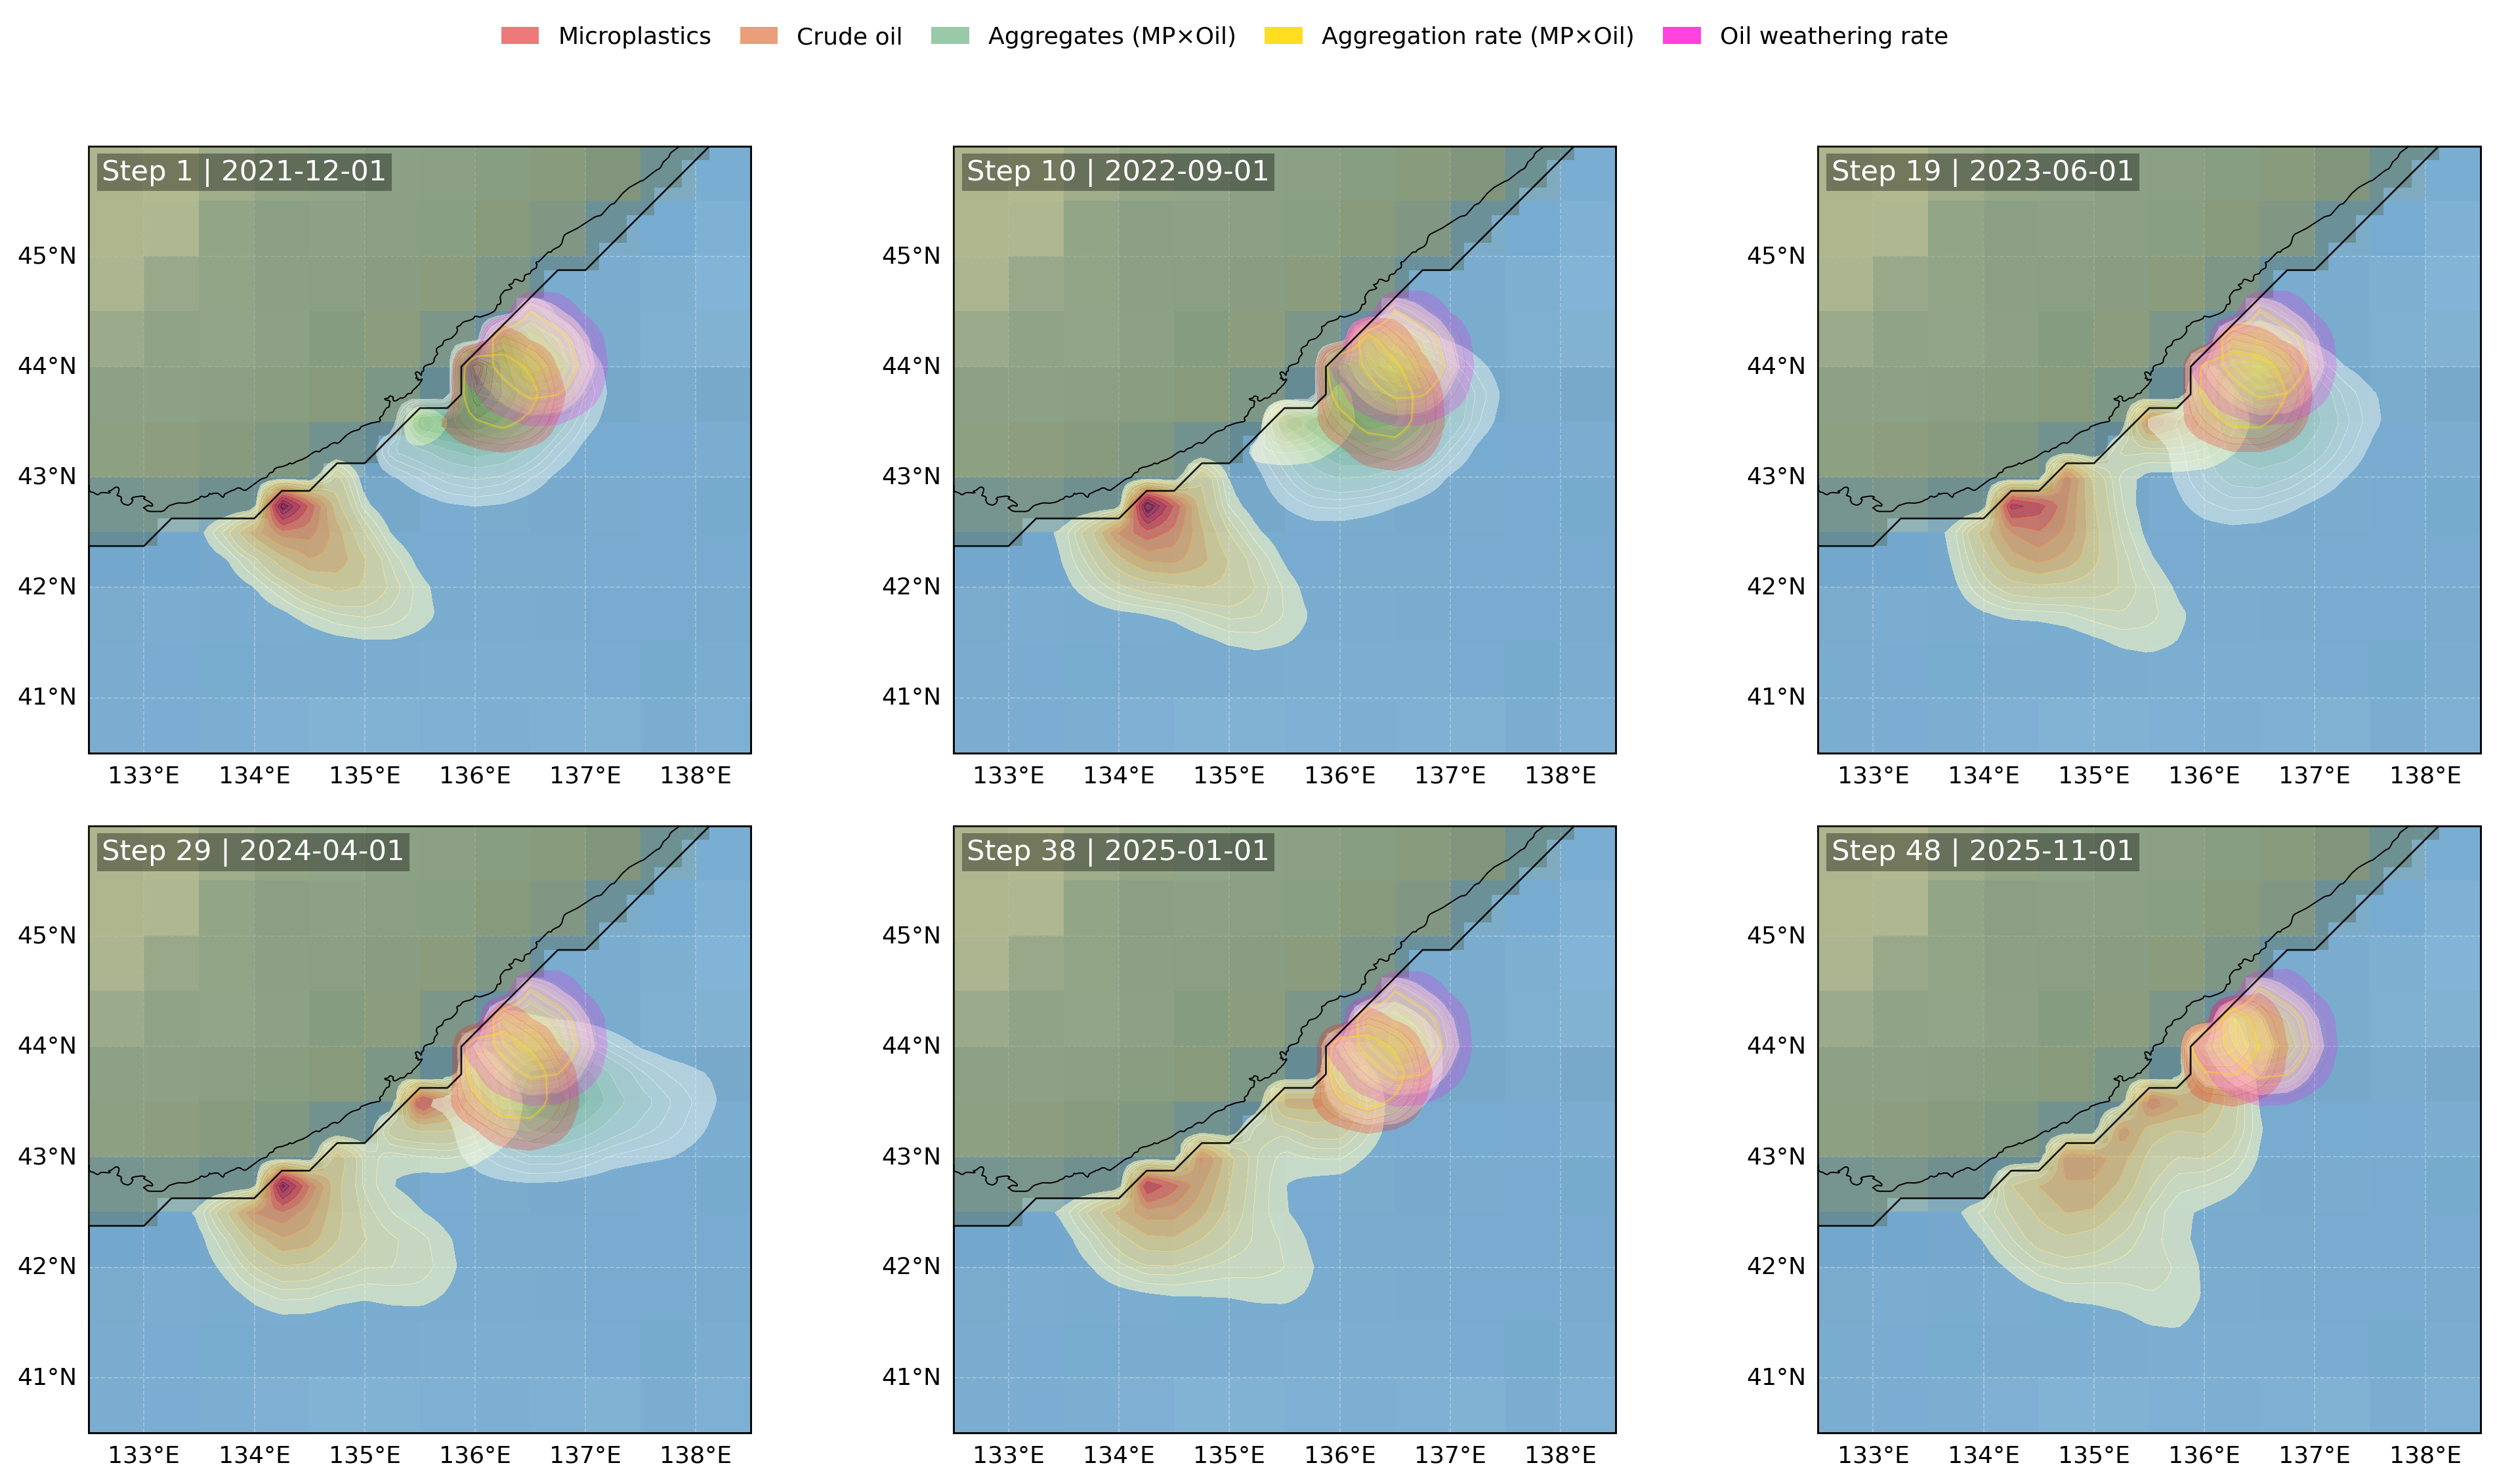
\includegraphics[width=0.98\textwidth]{figures/dataset_latest_multispecies_suite_seed03_panel.png}
\caption{Six sampled times from the dataset-driven surface multispecies proxy. The overlays show normalized microplastic, crude-oil, and aggregate fields together with aggregation and oil-weathering rates. The land mask blocks the proxy fields. Each species is normalized independently by its spatial maximum after every substep.}
\label{fig:app_multispecies}
\end{figure*}

The SPC presets use 12 sources, 8\,s dwell, and one required agent at medium difficulty; 6 sources, 6\,s dwell, and two required agents at hard difficulty.

\subsection{Optional Robot Operating System 2 (ROS 2) Jazzy bridge}

The bridge maps core $(x,y,z)=$(east, down, north) to the ROS East-North-Up (ENU) frame $(x,z,-y)$. External commands traverse the same clipping, dynamics, current, constraints, recorder, and task-update path as built-in controllers; internal-control mode can publish observations without accepting external motion commands.

\begin{table}[t]
\centering
\scriptsize
\setlength{\tabcolsep}{3pt}
\renewcommand{\arraystretch}{1.08}
\begin{tabularx}{\columnwidth}{l X}
\toprule
\textbf{Interface} & \textbf{ROS type and meaning} \\
\midrule
\texttt{/agent\_NNN/odom} & \texttt{nav\_msgs/Odometry}; ENU pose and velocity \\
\texttt{/agent\_NNN/current} & \texttt{Vector3Stamped}; ENU current \\
\texttt{/agent\_NNN/pollution} & \texttt{Float32}; local scalar probe \\
\texttt{/agent\_NNN/bathymetry} & \texttt{Float32}; positive water depth \\
\texttt{/agent\_NNN/cmd\_vel} & subscribed ENU velocity command \\
\texttt{/clock}, \texttt{/episode/metrics} & simulation time and JavaScript Object Notation episode state \\
\texttt{/reset}, \texttt{/step}, \texttt{/get\_task\_state} & \texttt{std\_srvs/Trigger} services \\
\bottomrule
\end{tabularx}
\caption{ROS 2 interface. Topic prefixes are \texttt{/oneocean/agents}; agent IDs are zero-padded.}
\label{tab:app_ros_contract}
\end{table}

The package was built and launched in a ROS 2 Jazzy container; topic discovery, frame conversion, one externally commanded step, state query, and reset completed successfully. ROS is an optional dependency.
